\section{Design Flow}
\label{sec:design-flow}

We propose a novel design flow for aspect-driven compilation of
dataflow designs to meet the following requirements and design goals,
addressing key areas in developing hardware acceleration solutions:
\begin{enumerate}
\item \emph{Performance:} specify high performance dataflow designs, that
  achieve significant speedup over software only versions; exploit the
  run-time reconfiguration capability of FPGA devices to improve
  performance and efficiency;
\item \emph{Portability:} improve portability of dataflow designs, to
  allow reuse of optimization strategies on various platforms;
\item \emph{Integration:} simplify translation of existing
  applications to high performance dataflow designs to facilitate the
  integration of the proposed design flow with existing (predominantly
  imperative) application code;
\item \emph{Productivity:} improve developer productivity by providing
  high-level means of specifying dataflow designs, controlling
  compilation strategies to reduce compilation time and generating
  boilerplate code automatically (e.g. for debug logging or
  simulation).
\end{enumerate}

We propose to address these requirements as follows:
\begin{itemize}
\item We introduce MaxC (described in Section \ref{sec:maxc}), a novel
  language for specifying dataflow designs that provides support for
  run-time reconfiguration. We specify the accelerated portion of the
  original applications using MaxC dataflow kernels;
\item By maintaining compatibility with the C99 standard we improve
  developer productivity by providing a familiar language and
  introduce the possibility of mixing hardware/software
  specifications;
\item By using an aspect driven compilation flow we decouple
  optimization from design development, improving design portability,
  and we automate the generation of code and design space exploration
  improving productivity. Finally, systematic design space exploration
  is used to identify maximum performance configurations, subject to
  platform specific constraints.
\end{itemize}



The proposed design flow is illustrated in Figure
\ref{fig:design-flow} and follows the steps described below:
\begin{enumerate}
\item The starting point is a C application containing an embedded
  high-level dataflow design. In our approach the latter is
  implemented using MaxC.
\item This is ``woven'' using the aspects in the aspect repository to
  generate new designs. The various categories of aspects are covered
  in more detail in Section \ref{sec:aspects}. For example the
  runtime reconfiguration aspect is responsible for partitioning and
  scheduling the application in a manner that achieves maximum
  performance. Design exploration aspects are used to control the
  design space exploration process based on feedback from the backend
  tools and user input (e.g. resource usage threshold)
\item Finally these are compiled using a backend compilation toolchain
  to FPGA designs. Our implementation uses MaxCompiler and translates
  the MaxC dataflow designs to MaxJ.  The feedback from the
  compilation process is used to drive the design space exploration
  process, repeating the weaving and compilation process until user
  specified requirements are met.
\end{enumerate}

Compared to existing work described
\cite{Cardoso:Teixeira:Alves:Nobre:Diniz:Cutinho:Luk:2012} and
\cite{cardoso2011new} our approach emphasises and provides more
freedom in the exploration of design level optimization (such as word
length optimizations and mapping of arithmetic blocks to DSPs) by
using a combination of implementation aspects (show in
\ref{fig:design-flow}) and MaxC optimization options.  Additionally
our approach targets a dataflow architecture as opposed to the von
Neumann architecture (GPP + Custom accelerator) proposed in the
related work. Finally, we explicitly consider and implement run-time
reconfiguration to achieve performance improvements.

\begin{figure}[!h]
%  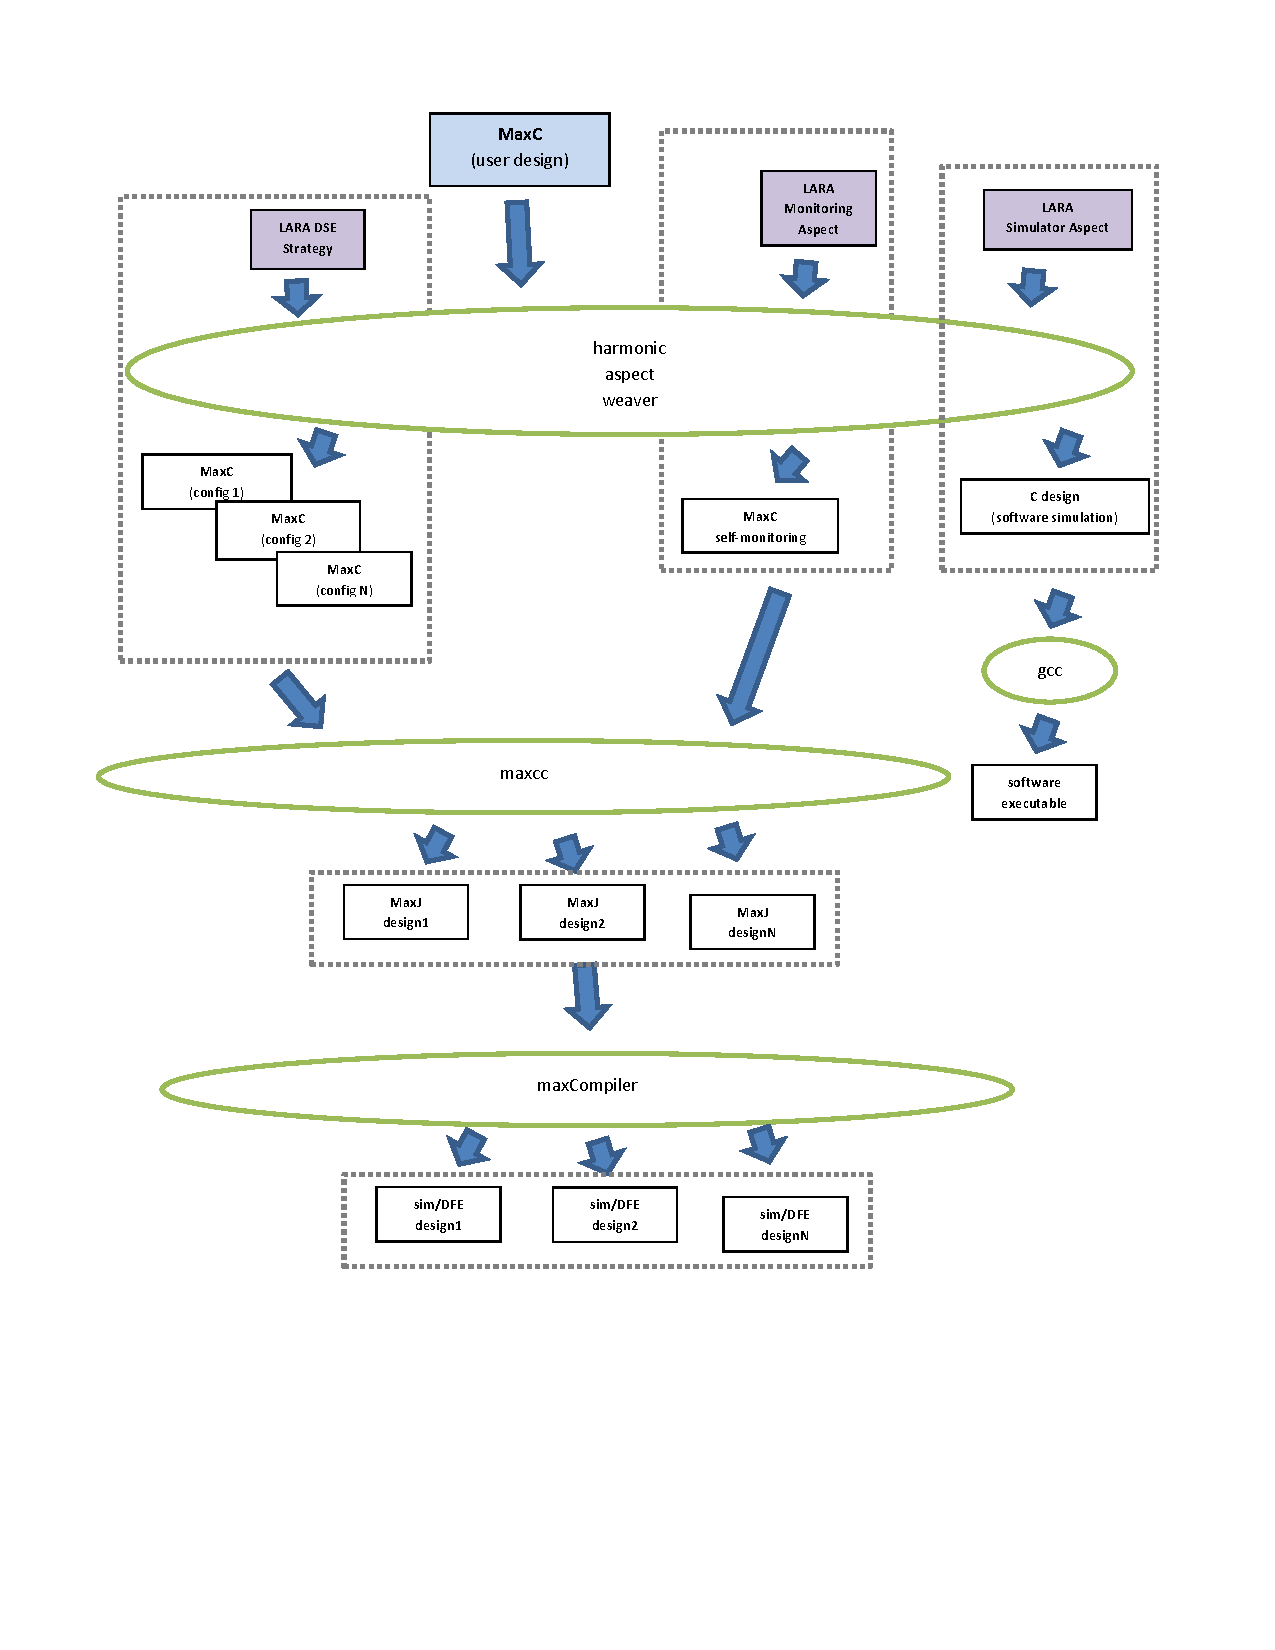
\includegraphics[scale=0.5, trim=50 180 0 50]{figs/lara_maxcc.pdf}
  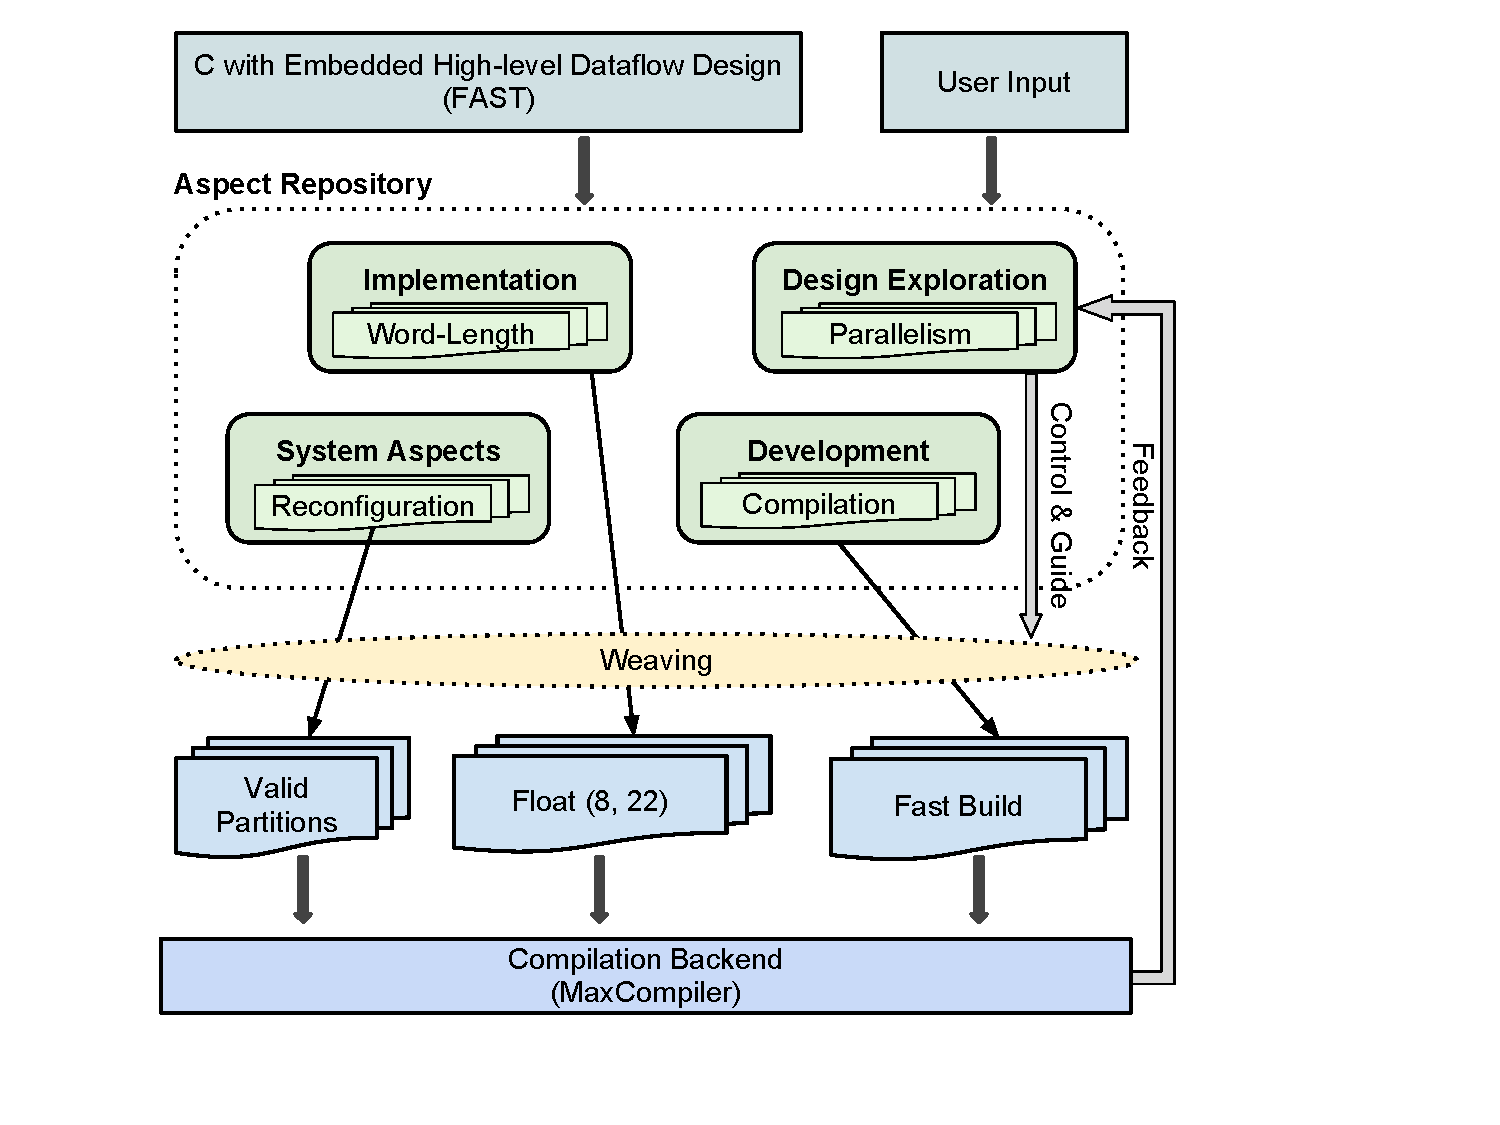
\includegraphics[scale=0.27, trim=0 0 0 0]{figs/design-flow}
  \caption{The proposed design flow.}
  \label{fig:design-flow}
\end{figure}
